\chapter{Client-Side File Hashing in the Web Browser}
\label{ch:browserhashing}
However, the decision to implement the frontend as a web application presents us with a challenge:
hashing the files to be signed client-side in the web browser itself.
If we had implemented "proper" client applications this would've been easy, but in a web browser and using its
JavaScript language not so much: it simply wasn't designed with file I/O and CPU-intensive cryptographic functions in mind.

The easiest solution would be to upload the files to be signed to the server and hash them there,
but this would be a clear violation of the least-information principle (the server doesn't need the file, only the hash)
and a breach of user privacy.
Nevermind the fact that signing large files could take a very long time over slow network connections,
and turn out to be quite expensive for mobile users billed for data by volume.

Another solution would be to ask the user to enter the file hashes instead of selecting files,
but this would be very user-unfriendly and most likely too much to ask from many users.

It is clear we must find a way to hash files in the web browser itself.
In order to achieve this we have found the following options:

\begin{enumerate}
    \item Using the browser-implemented \texttt{SubtleCrypto}~\cite{subtlecrypto} \gls{API}
    \item Using the \texttt{CryptoJS}~\cite{cryptojs} JavaScript implementation
    \item Using a \gls{WASM}-based implementation
\end{enumerate}

Each of these options comes with a number of advantages and disadvantages, as discussed in more detail in the following sections.

\subsection{Using SubtleCrypto}
\label{subsec:subtlecrypto}
The \texttt{SubtleCrypto} class offers the \texttt{digest(algorithm, data)} method~\cite{subtlecrypto}, which can be used to
calculate \gls{SHA-256} checksums.
The advantage of using this implementation is that it is available in all modern browsers\footnote{Where modern browsers means Mozilla Firefox, Google Chrome/Chromium, and Microsoft Edge, not older than the respective versions available in 2018},
and since it's executed with native code, being able to take advantage of \gls{AVX2} instructions, instead of JavaScript it should be quite fast.
There's a major drawback though: hashing a large amount of data progressively is not supported, the data has to be
passed to the function en bloc, as seen in listing~\ref{lst:subtlecrypto}.

\begin{lstlisting}[caption={Using SubtleCrypto for calculating SHA-256 checksums}, captionpos=b, language=JavaScript, label={lst:subtlecrypto}]
    crypto.subtle.digest("SHA-256", data).then(hash => {
    console.log(
    // convert ArrayBuffer to hex string
    Array.from(new Uint8Array(hash)).map(
    b => b.toString(16).padStart(2, '0')
    ).join('')
    );
    });
\end{lstlisting}
Our testing showed that selecting files larger than 200MB crashes Firefox tabs when trying to read their contents
into memory before we could pass it to the \texttt{digest} function.
If we assume the users will only ever select small files this should not pose a problem, but unfortunately it's not safe to assume this.

\subsection{Using CryptoJS}
\label{subsec:cryptojs}
\texttt{CryptoJS} does not have the limitation of \texttt{SubtleCrypto} and supports progressive hashing\footnote{
By progressive hashing we mean the ability to pass to the hash function the data piece by piece in order to avoid holding all of it in memory at once.},
as seen in listing~\ref{lst:cryptojsprogressive}.

\begin{lstlisting}[caption={Progressive SHA-256 hashing using CryptoJS},captionpos=b,language=JavaScript,label={lst:cryptojsprogressive}]
    const sha256 = CryptoJS.algo.SHA256.create();

    sha256.update("Message Part 1");
    sha256.update("Message Part 2");
    sha256.update("Message Part 3");

    const hash = sha256.finalize();
\end{lstlisting}

The advantage of using \texttt{CryptoJS} over \texttt{SubtleCrypto} is, as mentioned, the ability to hash piece-wise.
The disadvantage is that we need to load a third-party JavaScript library, using built-in functionality would be preferable.
And since JavaScript is an interpreted language, using it to calculate the checksums would result in significantly worse performance.
This is a problem especially on mobile devices limited in compute and memory resources as well as battery capacity.
Since we want to support mobile devices properly, and don't want to limit users to small files, we must do better.

\subsection{Using a WASM-based implementation}
\label{subsec:wasmhashing}
\gls{WASM} provides a low-level virtual machine in the web browser itself,
running machine-independent binary code, comparable to the \gls{JVM} or the \gls{CLR},
albeit much simpler and much less sophisticated.
By using this virtual machine we should be able to run code at near-native speed written in a statically-typed, compiled language such as Rust, C/C++ or Go.
Thus we expect significant performance gains over a JavaScript-based implementation.
While developing the \gls{WASM}-based hashing programmes, we encountered some interesting challenges, as described in the following paragraphs.

\paragraph{CORS Policy} While JavaScript can be executed simply by pointing the browser at a local \gls{HTML} file, the same doesn't work for \gls{WASM}.
The browser's security policy forbids it due to its \gls{CORS} rule~\cite{cors}.
We solved this by starting the \gls{HTTP} server built in to Go's standard library and having the browser load the \gls{WASM} binary through \gls{HTTP}.
The code is in appendix~\ref{chap:appendix_golangwebserver}.
For the Rust-based implementation we used the built-in web server of webpack~\cite{webpack}.

\paragraph{JavaScript/WASM Compatibility} The Golang project conveniently provides a file containing the necessary boilerplate code to load, start and interact with \gls{WASM} programmes called \texttt{wasm\_exec.js}.
But there's a catch: for each version of Go, the version of the accompanying \texttt{wasm\_exec.js} file used must match precisely.
If it doesn't, the code will crash with a segmentation fault.
It took us quite some time to figure out why the code we'd written only a few days prior would segfault now with no changes made to it.

\paragraph{Passing data} Functions written in Go intended to be used from the JavaScript side of things need to have a very specific signature.
As can be seen in listing~\ref{lst:funcsignaturewasm}, there is no typing: all arguments passed to the function are of type \texttt{js.Value} and the return value must be of type \texttt{interface\{\}}\footnote{This is Go's equivalent of Java's \texttt{Object}, it could be anything.}.
This posed us with the challenge of detecting the types and casting the data passed accordingly.

\begin{lstlisting}[caption={Golang WASM function signature}, captionpos=b, language=Go, label={lst:funcsignaturewasm}]
    func f(this js.Value, arg js.Value) interface{} {}
\end{lstlisting}

We've worked on this for hours, producing ugly reflection-based hacks, until we decided to just agree on the types of the arguments and return values beforehand despite the open function signature.
Now all that's needed is a little boilerplate to convert a JavaScript \texttt{Uint8Array} to a Golang \texttt{[]byte}, as seen in listing~\ref{lst:jscastingtogo}.

\begin{lstlisting}[caption={Uint8Array to {[]}byte}, captionpos=b, language=Go, label={lst:jscastingtogo}, captionpos=b]
    func progressiveHash(this js.Value, in []js.Value) interface{} {
    array := in[0]
    buf := make([]byte, array.Get("length").Int())
    js.CopyBytesToGo(buf, array)
    return this
    }
\end{lstlisting}

\paragraph{Goroutines} Go features its own concurrency primitive called Goroutines.
From a programmers' perspective, they can be used like threads, but they carry much less overhead.
Communication between goroutines is achieved by using so-called channels, which on a high level are comparable to queues.
Unfortunately, the \gls{WASM} specification wasn't drafted with this kind of concurrency in mind.
Go is forced to unwind and restore the call stack when switching between goroutines, which is very expensive~\cite{lolnogoroutines}.
We rewrote the Go programme to work without them, and we've seen a small but significant performance improvement.

\paragraph{Rust based WASM}
As the Go implementation also includes the Go runtime,
which makes the wasm file much larger,
and starts a programme that will run continuously in the background it isn't the optimal choice for creating a WebAssembly implementation.
As neither of us knows any other of the other languages that compile to WebAssembly well, we excluded them at first.
However with the drawbacks of the Go based implementation we decided to try to implement a Rust-based version as well,
in order to see how they compare both in performance and ease of development.


\subsection{Performance Comparison}
\label{subsec:perfcomphashing}
No one likes waiting for slow software to do its work, and neither do we.
This is why we decided to compare the performance of the aforementioned options in a simple test:
we measure the time it takes for the browser to calculate the checksum of 1GB of random data using the aforementioned methods.
The code used for each example is in appendix~\ref{ch:appendix-in-browser-hashing-code}.
The tests were run on Debian 10 using Firefox 69 on an Intel i7-8550U.
The results can be seen in figure~\ref{fig:hashingperformance}.

As expected, the in-browser \texttt{SubtleCrypto}-implementation is the fastest, followed by the Rust-based implementation.
JavaScript is so ridiculously slow it's not even trying to compete.
In order to provide a reference to compare the hashing speeds to we include the performance of the \texttt{openssl} command-line programme.

\begin{figure}
    \begin{center}
        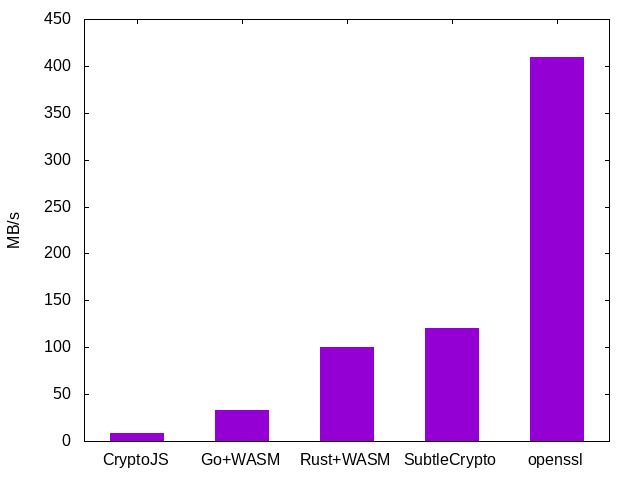
\includegraphics[width=0.7\linewidth]{images/hashingperformance.png}
        \caption{Hashing speed in MB/s (higher is better)}
        \label{fig:hashingperformance}
    \end{center}
\end{figure}


\subsection{Deciding On The In-Browser Hashing Implementation}
\label{subsec:deciding-on-the-in-browser-hashing-implementation}
It is clear from figure~\ref{fig:hashingperformance} that \texttt{SubtleCrypto} is the fastest of the options we tried.
Unfortunately, since it doesn't support piece-wise hashing we're forced to pick the next-fastest option,
the Rust-based implementation running in the \gls{WASM} \gls{VM}.

